
\documentclass{article}
\usepackage{amsmath, amsfonts, amssymb, amsthm} %packages for math-related
\usepackage[margin=1.2in]{geometry}
\usepackage[shortlabels]{enumitem}
\usepackage[utf8]{inputenc}
\usepackage{graphicx} % package for inserting images
\usepackage{commath} % package for things like \del, \cbr, and \sbr. These handle parentheses well.
\usepackage[mathscr]{euscript}%for \scr command 
\usepackage{../commands} %package with all of the commands for this class
\usepackage{url}
\setlength{\parindent}{0em} % so paragraphs aren't indented
\newcommand{\lcm}{\text{lcm}}
\newcommand{\Hom}{\text{Hom}}
\newcommand{\Ann}{\text{Ann}}

% ********************************************************** %
%               THINGS TO EDIT BELOW THIS LINE               %
% ********************************************************** %
\newcommand{\D}{\nabla}
\renewcommand{\d}{\partial}
\usepackage{wrapfig}
\title{\textsc{MATH 173 Problem Set 2}}
\author{Stepan (Styopa) Zharkov}
\date{April 13, 2022}
\begin{document}
\maketitle
\problem{1} Solve the equation $u_x+ \cos xu_y= y, u(0, y) = y$. Sketch the characteristic
curves. \tri
\hop
\solution
This is a semilinear PDE and can be solved with the same methods as last week. Let 
Let $(x(s), y(s))$ be a characteristic curve. We see that $x'(s) = 1, y'(s) = \cos$ with $x(0) = 0$. 
\hop
Solving this, we get that $x(s) = s, y(s) = \sin(s) + a$. Let $f_a(s) = (s, 
\sin(s)+a)$ be the characteristic curve. Also, let $\omega_a(s) = u(f_a(s))$.  We know $\omega_a'(s) = y(s) = \sin(s) + a$ and $\omega_a(0) = a$. So, we see that $\omega_a(s) = -\cos(s)+as +a +1$. We see that $x= s$, $y= \sin(s)+a$. Solving for $a, s$, we have that $s =x$ and $a = y - \sin(x) + y$. Thus,
\[u(x,y) = \omega_a(s)=-\cos(s)+as +a +1 = -\cos(x)+xy - x\sin(x)+y-\sin(x)+1.\]
We can check that this solution fits $u_x +\cos(x)u_y = y$ indeed. 
\qed
\begin{center}
    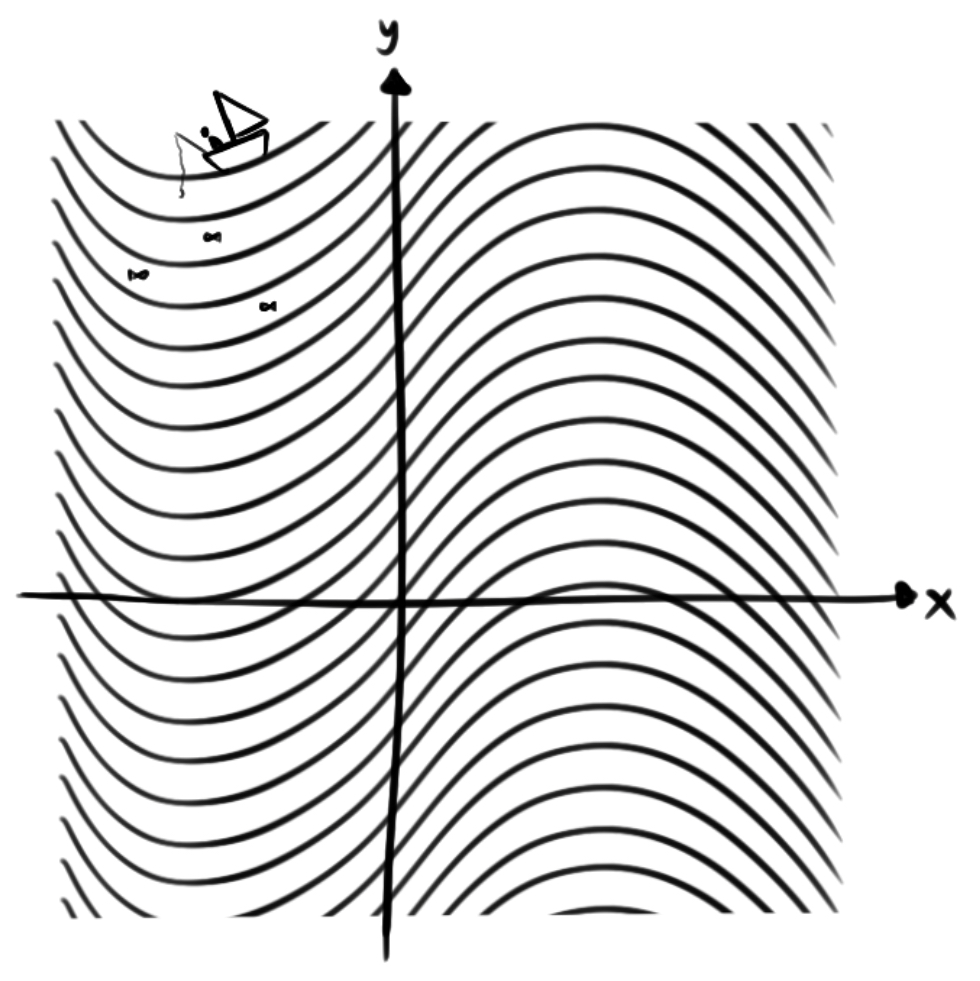
\includegraphics[width=6cm]{../images/waves.jpeg}
  \end{center}


\newpage
\problem{2}
\begin{enumerate}[(a)]
    \item Solve the equation $u_t+ \sqrt{u}u_x= 0, u(0, x) = x^2$.
    \item  Draw the (projections) of some of the characteristic curves to the $(t, x)$-plane. Find the
    largest $T$ such that the solution exists in $C^1((0, T ) \times 
    \RR)$.
\end{enumerate}
\tri 
\hop 
For this question, we will answer both parts (a) and (b) together because we must go through the ideas to solve part (b) to be able to find the solution in (a) anyway. This is a quasilinear PDE that can be solved by finding the characteristic curves in 3-dimensional space, as discussed in chapters 3 and 4. 
\hop 
Let $(t(s), x(s), z(s)$ be the characteristic curve on the graph of $u(t,x)$. We see that $t'(s) = 1, x'(s)=\sqrt{z(s)}, z'(s) = 0$ and that the initial conditions give us $t(0)=0, z(0)= x(0)^2.$ Solving this, we have that $t(s)=s, z(s)=a$ and $x(s) = s\sqrt{a} \pm \sqrt{a}$ for some constant $a\ge0$. Let $\omega^+_a(s) = (s, s\sqrt{a} + \sqrt{a}, a)$ and $\omega^-_a(s) = (s, s\sqrt{a} - \sqrt{a}, a)$ be the characteristic curves. Note that $\omega^+_0$ and $\omega^-_0$ are the same curve. When projected onto the $(x,y)$ plane, the curves look as follows:
    \begin{center}
      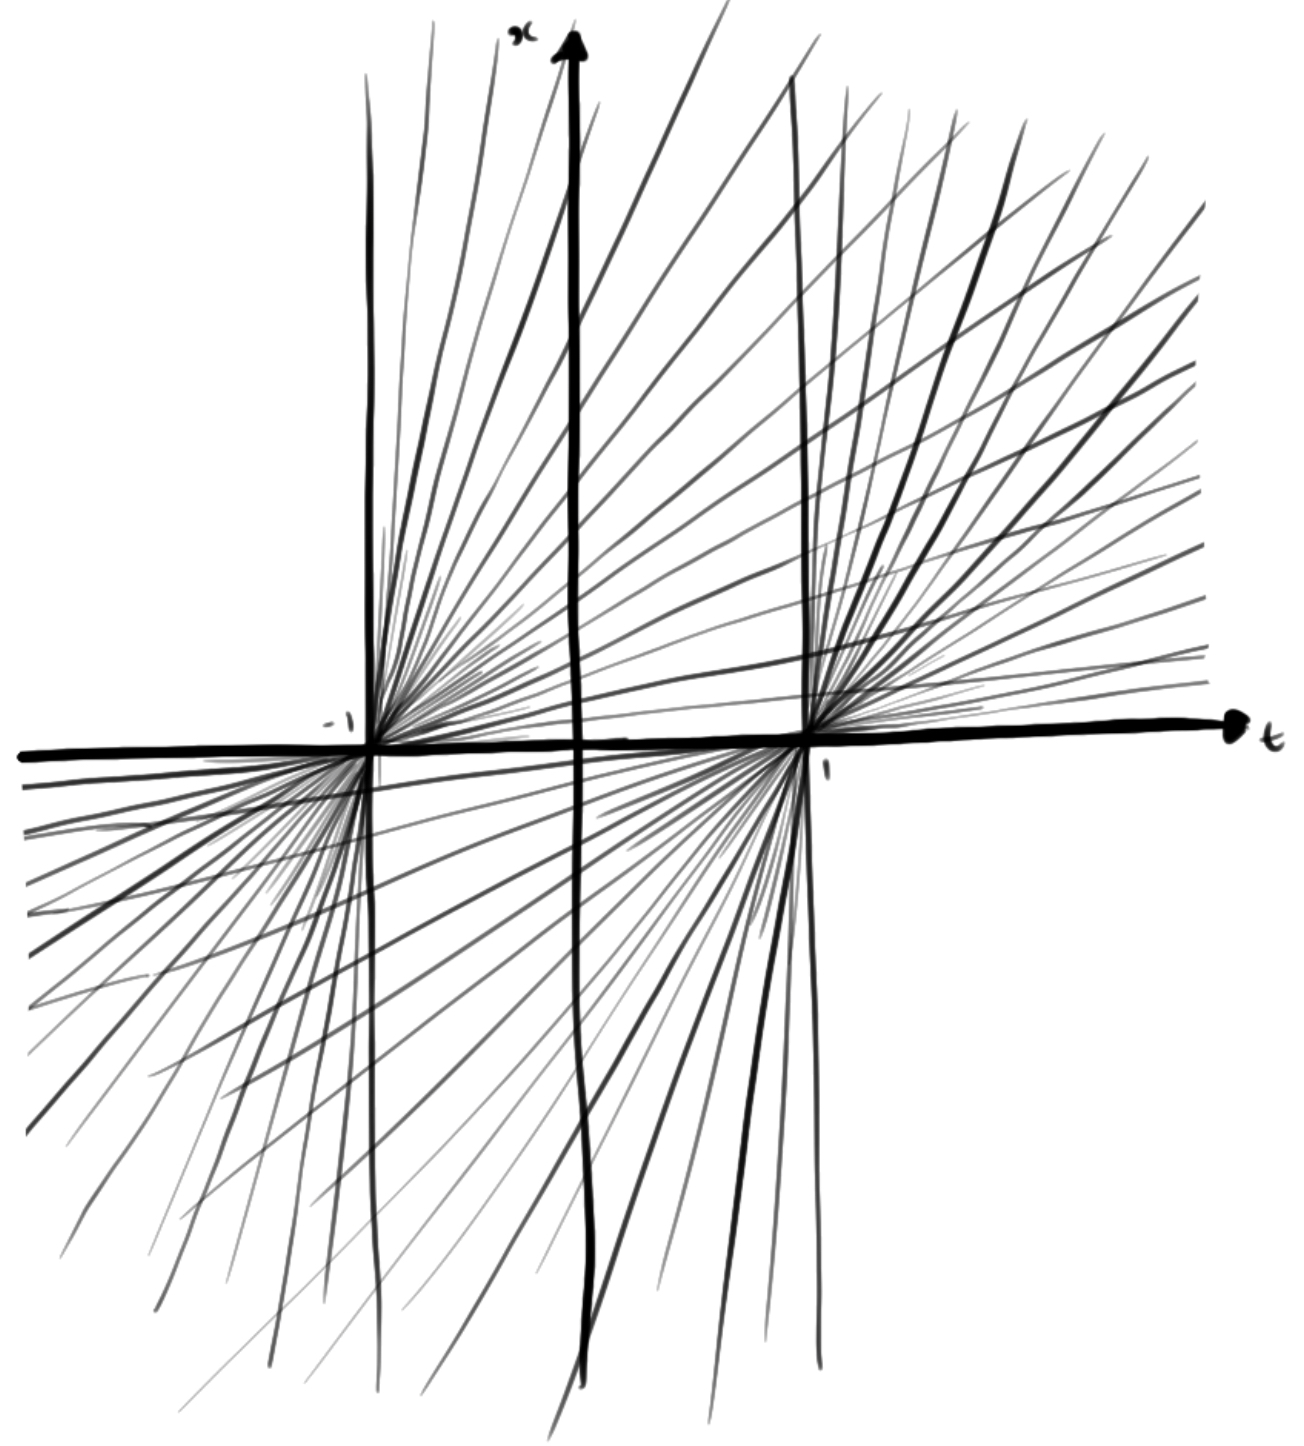
\includegraphics[width=4.2cm]{../images/sqrts.jpeg}
    \end{center}
The value of $u$ is constant and equal to $a$ along each curve. We see that in the region where $|t| > 1$, the curves either intersect or do no pass through at all. For the region $|t| < 1$, we can find a solution. Namely, we see that $t= s$ and $x = s\sqrt{a} \pm \sqrt{a}$, so we can solve to see that any $(x,t)$ where $t < 1$ and $x \ne 0$ can be uniquely expressed by setting 
\[s= t, a = \begin{cases}
    \del{\frac{x}{t+1}}^2 &\text{ if } x\ge  0 \\
    \del{\frac{x}{t-1}}^2 &\text{ if } x\le 0.
\end{cases}\]
Note that since $\omega^+_0$ and $\omega^-_0$ are the same curve with $a=0$, we do not have any problems at 0. Since $u(t,x) = z(s) = a$, we can see that  
\[u(t,x) = \begin{cases}
    \del{\frac{x}{t+1}}^2 &\text{ if } x\ge  0 \\
    \del{\frac{x}{t-1}}^2 &\text{ if } x\le 0.
\end{cases}\]
is our solution fo $|t|<1$. To finish answering part (b), we see that for $T=1$, our expression is continuously differentiable on $[0,T] \times \RR$. The only thing we have to check for this is that the derivatives near $x = 0$ match up, but we see that $u_x$ approaches $0$ from both sides, so we can continue.
\hop 
Finally, we can check that for any $T>1$, we encounter problems. The characteristic curves $\omega_0^-$ and $\omega_1^-$ pass through the same point $1, 0$, but with different values of $a$, so any solution must be equal to both $0$ and $1$ at that point, which is impossible. Thus, $T=1$ is the largest choice we could have made. \qed
\hop


\newpage
\problem{3} We consider a system of first order ODEs:
\[x'_j(t) = a_j(t, x(t)), x(t) = (x_1(t), \dots, x_n(t)),\]
with the initial condition $x(0) = x_0$. Suppose that $|a_j(t, x) - a_j(t, y)| \le M |x -y|$. Show that
for some $t_0$ there is a unique solution $x : (-t_0, t_0) \to \RR^n$ to this equation in $C^1((-t_0, t_0), \RR^n)$. \tri
\hop
\solution
This problem is literally given to us by theorem 3.5 in the notes. However, we will elaborate a little on the proof of that theorem instead of writing ``true by theorem 3.5''. 
\hop 
Instead of thinking about this as a system of ODEs, let's think of it as one ODE 
\[x'(t) = a(t,x(t)), x(t) = x_0(t)\]
in a larger space, where $a(t,x(t)) = (a_1(t,x(t)), \dots, a_n(t,x(t))$. Let $t_0 < \frac{1}{nM}$. Consider the map $T: C^0((-t_0, t_0), \RR) \to  C^0((-t_0, t_0), \RR)$ where
\[Tx(t) = x_0 + \int_0^ta(\tau,x(\tau))d\tau.\]
We see that 
\begin{align*}
    d(Tx,Ty) &= \sup_{t \in (-t_0,t_0)}\cbr{\norm{\del{x_0 + \int_0^ta(\tau,x(\tau))d\tau}-\del{x_0 + \int_0^ta(\tau,y(\tau))d\tau}}}\\
    &= \sup_{t \in (-t_0,t_0)}\cbr{\norm{\int_0^t\del{a(\tau,x(\tau))-a(\tau,y(\tau))}d\tau}}\\
    &\le \sup_{t \in (-t_0,t_0)}\cbr{\int_0^t\norm{a(\tau,x(\tau))-a(\tau,y(\tau))}d\tau}\\
    & \le  \sup_{t \in (-t_0,t_0)}\cbr{\int_0^tnM\norm{x(\tau)-y(\tau)}d\tau} \\
    & \le  \sup_{t, s \in (-t_0,t_0)}\cbr{\int_0^tnM\norm{x(s)-y(s)}d\tau} \\
    & \le  \sup_{t, s \in (-t_0,t_0)}nM\norm{x(s)-y(s)}\cbr{\int_0^t1d\tau} \\
    & \le  \sup_{s \in (-t_0,t_0)}nM\norm{x(s)-y(s)}t_0\\
    & \le nMd(x,y)t_0\\
    & < d(d,x).
\end{align*}
Thus, $T$ is a contraction mapping over a complete space, so it has a unique fixed point $x$ such that 
\[x(t) = x_0 + \int_0^ta(\tau,x(\tau))d\tau,\]
so $x$ is the unique solution to $x'(t) = a(t,x(t)), x(t) = x_0(t)$ by the fundamental theorem of calculus. Note that $a$ is continuous so, $x'$ is continuous, so $x$ is $C^1$. So, our system of equations has the same $x$ as its unique solution. 
\qed


\newpage
\problem{4}Suppose that $u_t+ (F (u))_x= 0, u(0, x) = g(x)$, where $F \in C^2(\RR), g \in C^1(\RR)$
and $u \in C^1((0, T ) \times \RR) \cap C([0, T ] \times \RR)$.
\begin{enumerate}[(a)]
    \item Show that the method of characteristic gives $u(t, x) = g(x - F'(u(t, x))t)$.
    \item Show that the formula in part (a) holds for all $0 \le t \le T, x \in \RR$. 
\end{enumerate}
\tri
\hop
\solution
\begin{enumerate}[(a)]
    \item We can approach this as we approached conservation laws in class. As always, let $(t(s), x(s), z(s))$ be a characteristic curve on the graph of $u$. From our derivation in class, we know that $t(s) = s, x(s)= F'(g(a))s + s$, and $z(s) = g(a)$ for the parameter $a$. So, all the characteristics are straight lines and $u$ is constant along them. Rearranging our expressions, we see that $s = t$ and $a = x - F'(g(a))t$. Plugging this in, we see that 
    \[u(t,x) = z(s) = g(a) = g(x - F'(g(a))t) = g(x - F'(u(t,x))t),\]
    as we wanted.  \qed
    \item For this problem, we know that a solution $u$ exists, and we know that the equation from part (a) is satisfied on the characteristic curves on some solution, so it would suffice to show that the characteristic curves go through every point in $[0,T] \times \RR$ and that they don't intersect. 
    \hop
    First, let us show that the characteristic curves don't intersect. We know the value of $u$ is constant along the characteristic curves. So, if two curves with parameters $a_1, a_2$ where $a_1 \ne a_2$ defined as in part (a) intersect, then $g(a_1) = g(a_2)$. However, we see that the slopes of the projection of both of these characteristic curves onto the $(t,x)$-plane are  $F'(g(a_1)) = F'(g(a_2))$. So, the projection curves cannot intersect without them being the same curve.
    \hop 
    Now, let's use the fact that the projection curves can't intersect to argue that every point is covered. Let $b$ be the slope of the characteristic projection starting at $(0,0)$. For an arbitrary point $(t,x) \in (0,T) \times \RR$ above that characteristic projection, consider the line going through $(t_0,x_0)$ and $(T,Tb)$. Let that line cross the $x$-axis at $(0,c)$. Now, intuitively, we see that the characteristic curve projection starting at $(0,c)$ cannot go underneath the point $(t_0,x_0)$ or else it will cross our first characteristic curve projection . More formally, let $(t,x(t))$ be the projection starting at $(0,c)$. We see that if the slope is less than $(Tb-x_0)/(T-t)$, then $x(T) < b$, so this curve intersects our initial curve. So, the slope is more than $(Tb-x_0)/(T-t)$ and thus $x(t_0) > x_0$. 
        \begin{center}
          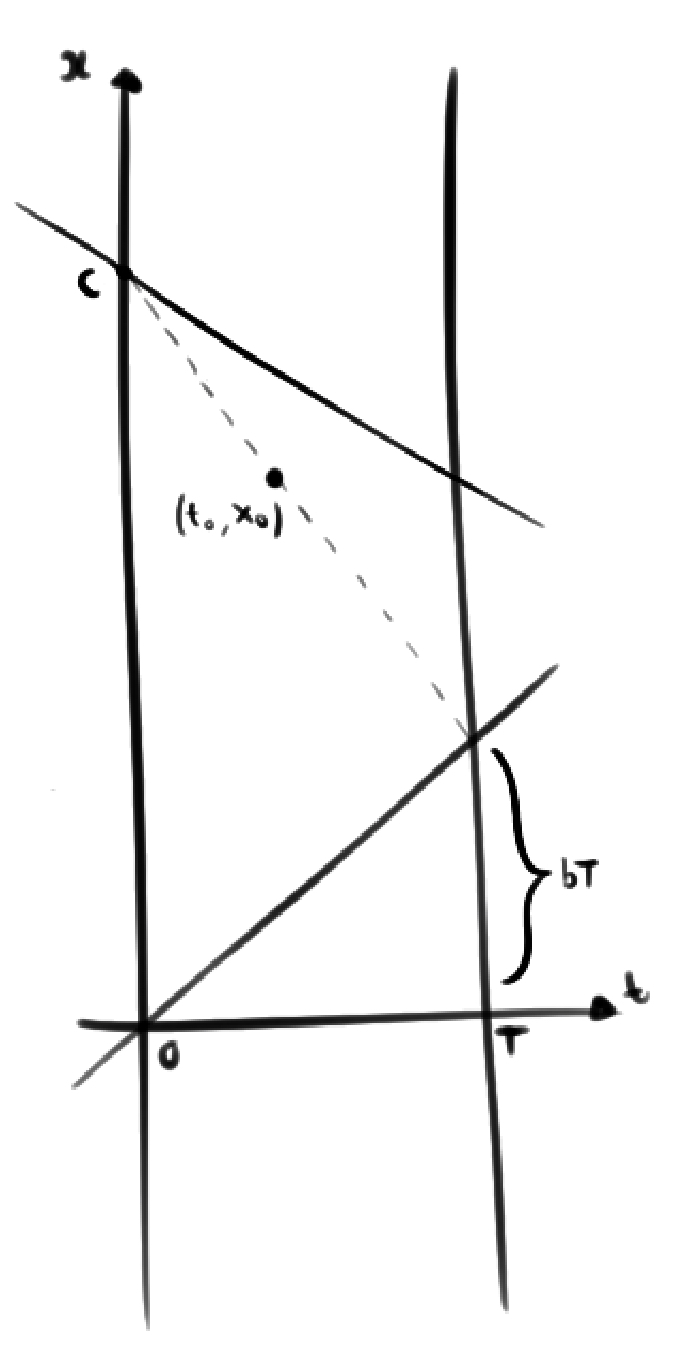
\includegraphics[width=3.5cm]{../images/roof}
        \end{center}
    Consider the map $f(a) = a + F'(g(r))t_0$. This is the map that gives the $x$-value of the characteristic projection with parameter $a$ at $t_0$. We see that $f(0) = t_0b < x_0$ and $f(c) \ge x_0$. Since $f$ is continuous, by the intermediate value theorem, there is a $d$ such that $f(d) = x_0$. This means that the characteristic curve projection starting at $(0,d)$ passes through $(t_0,x_0)$, as we wanted. 
    \hop 
    For points $(t_0, x_0)$ below the initial curve, we can define $c$ and $x(t)$ in the exact same way. We see that $x(t_0)$ must be no more than $x_0$, so $f(0) = t_0b > x_0$ and $f(c) \le x_0$. Again by the intermediate value theorem, there is some $d$ such that $f(d) = x_0$. This means that the characteristic curve projection starting at $(0,d)$ passes through $(t_0,x_0)$. 
    \hop 
    So, any point on the $(t,x)$-plane has a characteristic curve projection passing through it, so we can conclude that the equation from part (a) holds on all of $(0,T) \times \RR$. \qed
\end{enumerate}


\newpage
\problem{5}  Let $u$ and $g$ be as in Problem 4. Assume also that $g(x) = 0$ when $|x| > R$ for
some $R$.
\begin{enumerate}[(a)]
    \item Prove that there exists a constant $C$ such that $u(t, x) = 0$ when $|x|> R + Ct$.
    \item Prove the following conservation law:
    \[\int_\RR u(t, x)dx = \int_\RR g(x)dx, 0 \le t \le T.\]
\end{enumerate}
\tri
\hop
\solution
\begin{enumerate}[(a)]
    \item We see that $u$ is constant along the characteristic curves, so the value of $u$ is $0$ along any curve that starts at $(0,x)$ for $|x| > R$. We see that the slope of the projection onto the $(t,x)$-plane is $\frac{F'(g(a))}{1} = F'(g(a))$ for the curve that starts at $(0, a, g(a))$. Since $F'(g(a))$ is continuous on $[-R, R]$, we can let $C > \sup \{F'(g(a)) : |a| \le R \}$. Then, the projections of the characteristics starting at $(0,a)$ for $|a| \le R$ are limited to the region $\{(t,x): |x| \le R+Ct\}$. So, any point outside this region must be on a characteristic starting at  $(0,a)$ for $|a| > R$ and thus $u$ has a value of 0 there, which is what we wanted to prove. \qed 
    \begin{center}
        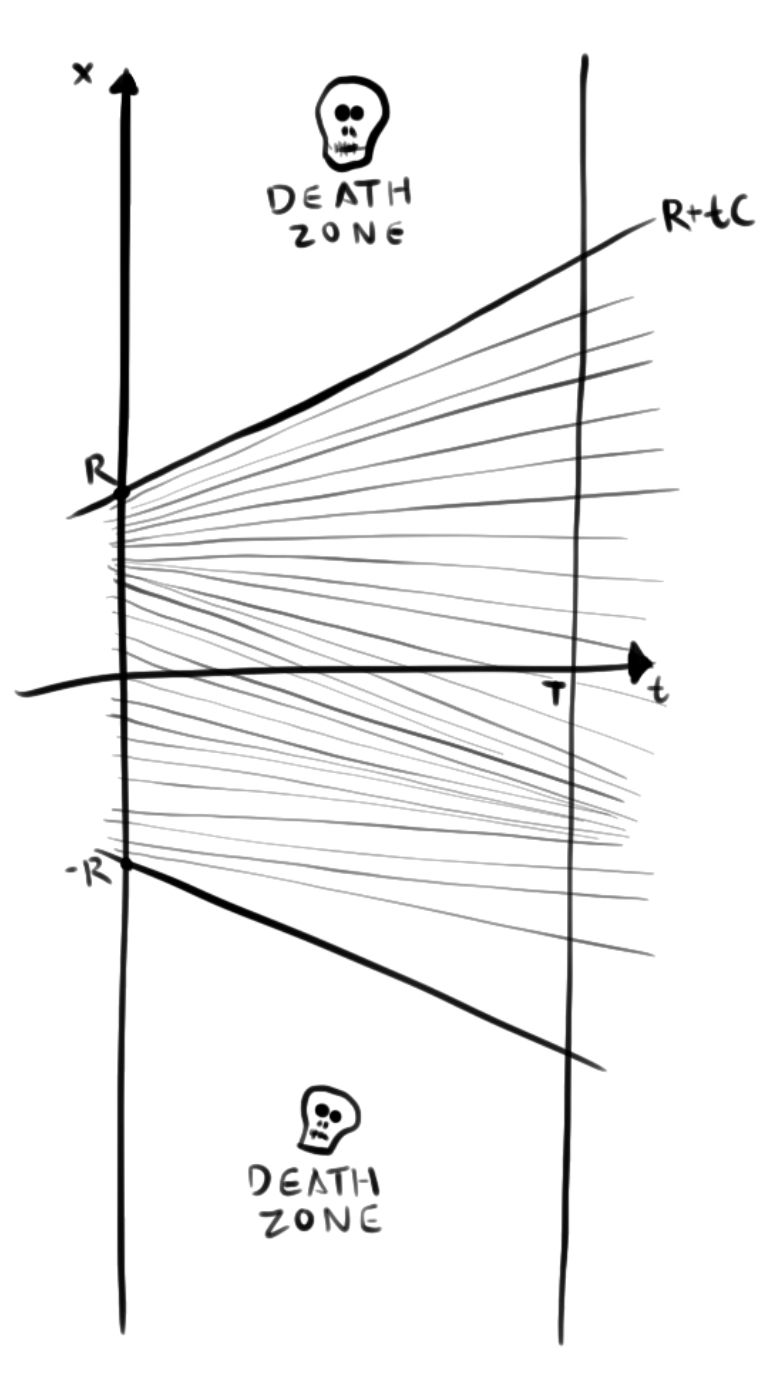
\includegraphics[height=6.3cm]{../images/death-zone.jpeg}
    \end{center}
    \item This problem essentially explains why conservation laws are called conservation laws. The ``total mass of $u$'' (i.e. the integral) of stays constant over time, as explained in the notes (page 5 of chapter 4).
    \hop 
    For $t = 0$, we see that 
    \[\int_\RR u(t,x)dx = \int_\RR g(x) dx\]
    by definition. For $t \in (0,T)$, we see that since $u$ is $C^1$, 
    \[\d_t\int_\RR u(t,x)dx = \int_\RR u_t(t,x)dx = -\int_\RR F(u(t,x))_x dx  =  -\lim_{x \to \infty}( F(u(t,x)) - F(u(t,-x)))= -F(0) +F(0) =0.\]
    by the fundamental theorem of calculus and the fact that $u(t,x)$ vanishes for large enough $x$ by part (a). 
    \hop
    So, we see that $\int_\RR u(t,x)dx$ is indeed constant as a function of $t$. Since it is continuous, we can extend to the endpoint at $T$ as well and conclude that 
    \[\int_\RR u(t,x)dx = \int_\RR g(x) dx\]
    for all $t \in [0,T]$, as we wanted. \qed
\end{enumerate}


\newpage
\problem{6} Use the Rankine–Hugoniot condition to find a solution to the Burgers equation
$u_t+ uu_x= 0$ with the initial condition
\[u(0, x) = \begin{cases}
    0, x &< 0,\\
1, x &> 0
\end{cases}\]
which is piecewise constant and take values 0, 1/2, and 1.
\tri
\hop
\solution
This problem is similar to the example with only 1 and 0 in the range that we did in class, but we have to insert $1/2$ in between the two regions.
\hop 
Let $h(t)$ be a border between two constant value regions and $a_+, a_-$ be the values in the two regions. If $u$ is a weak solution, then by the Rankine-Hugoniot condition, we have $(a_+-a_-)h'(t) = a_+^2/2-a_-^2/2$. Since we assume that the values are different, we can divide by $a_+-a_- \ne 0$, so $h'(t) = (a_++a_-)/2$. Thus, we see that $h(t)= (a_++a_-)/2 \cdot t$. For $(a_+,a_-)$ set to $(0,1), (1/2, 1)$, and $(0, 1/2)$, we see $h(t)$ must be a line with a slope of $1/2, 3/4$, and $1/4$ respectively. Note that the order of $a_+,a_-$ does not change the slope. Since the problem asks that all 3 values are in the range, and we know that $u(0,x)$ is 0 below $x=0$ and 1 above, we can conclude that the only possible option satisfying the R-H condition. Namely, 
\[u(t,x)= \begin{cases}
    0 &\text{ if } x <  \frac{1}{4}y \\
    1/2 &\text{ if } \frac{1}{4}y \le x \le  \frac{3}{4}y \\
    1 &\text{ if }x > \frac{3}{4}y.
\end{cases}\]
We see that constant functions satisfy $u_t + uu_x=0$ and our function satisfies the jump condition, so it is indeed a weak solution. \qed
\begin{center}
    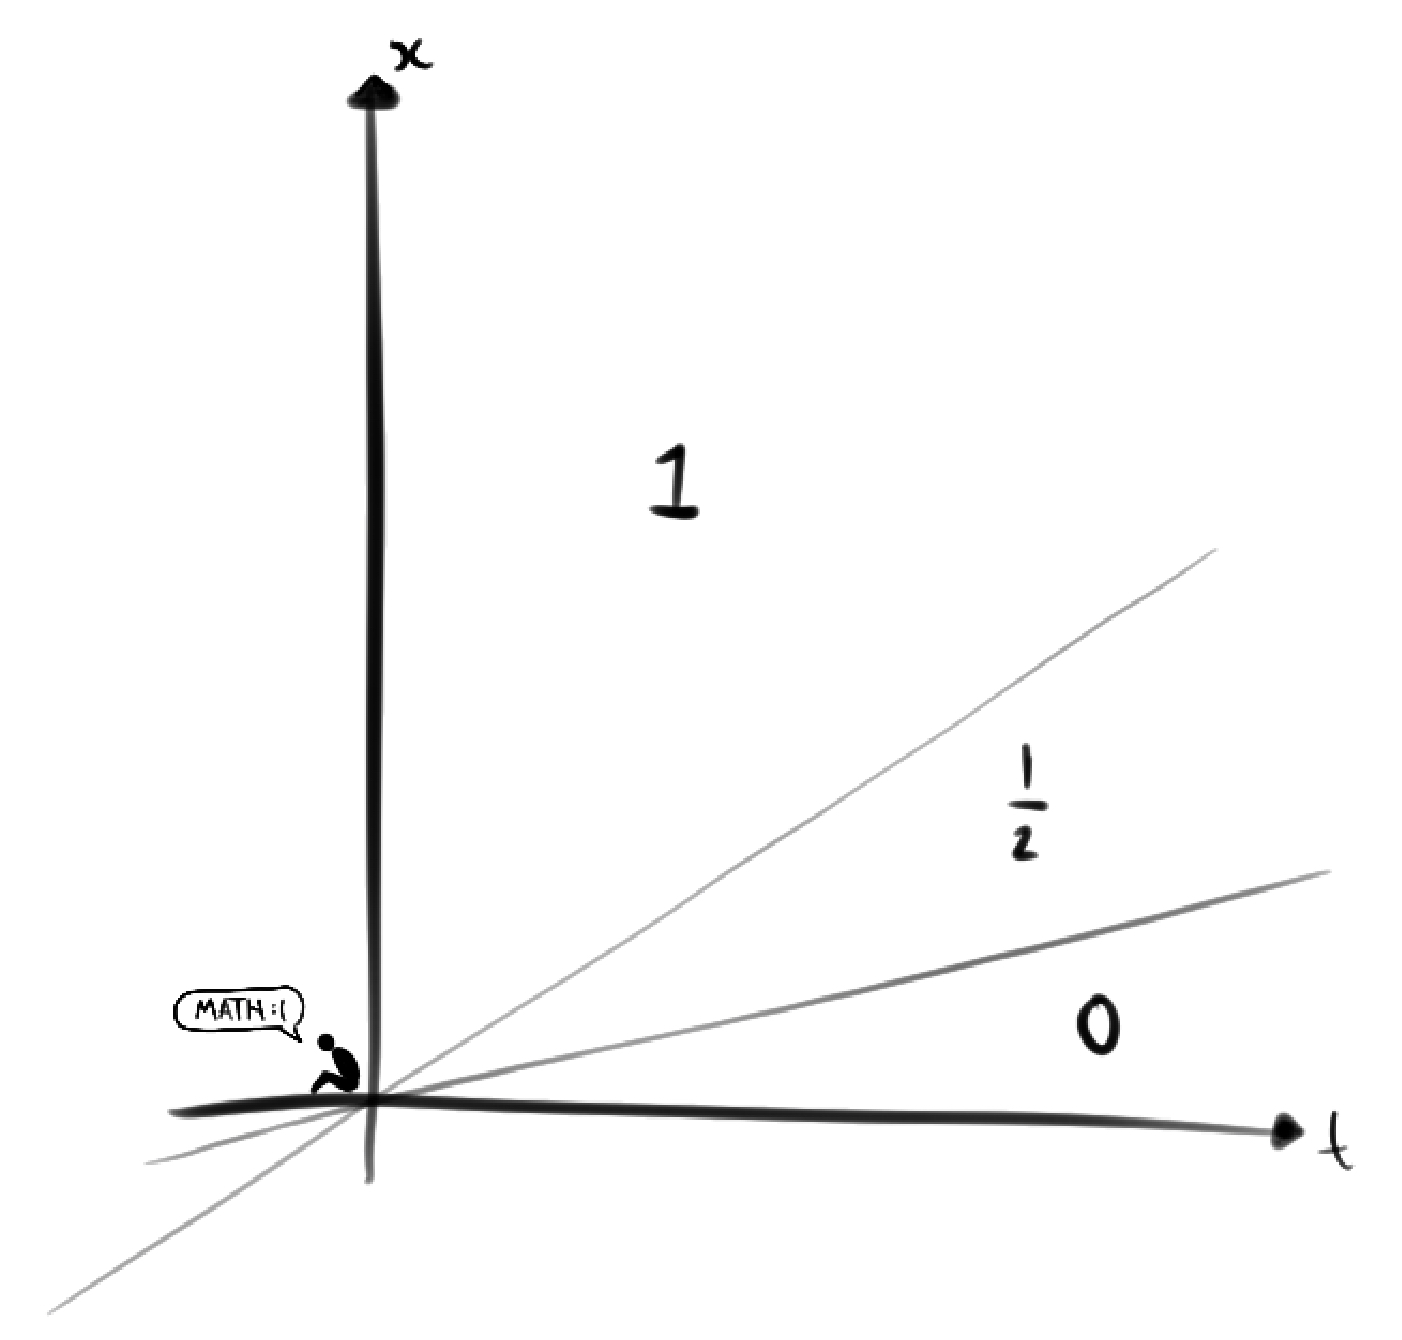
\includegraphics[height=5cm]{../images/one-half}
\end{center}
\newpage
\problem{7} Consider the conservation law $u_t+ (F (u))_x= 0, u(x, 0) = g(x)$, where $F \in
C^2(\RR)$. Let $v(t, x) = F'(u(t, x))$.
\begin{enumerate}[(a)]
    \item Show that if $u \in C^1$ then $v \in C^1$ and $v$ satisfies Burgers' equation.
    \item Suppose that $u$ is a weak solution to the conservation law, $u$ has a jump discontinuity
    along a curve, and is $C^1$ otherwise. Does this imply that $v = F '(u)$ is a weak solution to the
    Burgers equation?
\end{enumerate}\tri
\hop
\solution
\begin{enumerate}[(a)]
    \item Let $v(t,x) = F'(u(t,x))$. We see that since $u_t(t,x) + F'(u(t,x))u_x(t,x) = 0$, we know 
    \begin{align*}
        v_t + vv_x &= \d_tF'(u(t,x)) + F'(u(t,x))\d_xF'(u(t,x))\\
        &= F''(u(t,x))u_t(t,x) + F'(u(t,x))F''(u(t,x))u_x(t,x) \\
        &=F''(u(t,x))(u_t(t,x) + F'(u(t,x))u_x(t,x))\\
        &= 0.
    \end{align*}
    So, by definition, $v$ satisfies Burgers' equation. \qed
    \item No, the implication doesn't hold. Let $F(x) = x^3$. Then, the equation becomes $u_t + 3u^2u_x = 0$. Consider the function 
    \[u(t,x) = \begin{cases}
        0 \text{ if } x \le t \\
        1 \text{ if } x > t.
    \end{cases}\]
    We see that the constants satisfy $u_t + 3u^2u_x = 0$. Also, on the boundary $h(t) = t$, we see that $(1-0)h'(t) = 1^3 - 0^3$, so the Rankine-Hugoniot condition is satisfied. Thus, $u$ is a weak solution. However, we see that 
    \[v(x,t) = 3u^2(t,x) = \begin{cases}
        0 \text{ if } x \le t \\
        3 \text{ if } x > t.
    \end{cases},\]
    which does not satisfy the Rankine-Hugoniot condition for Burgers' function because for the boundary $h(t) = t$, we see $h'(t) = 1 \ne 3/2 = 3/2+0/2$. \qed 
    \begin{center}
        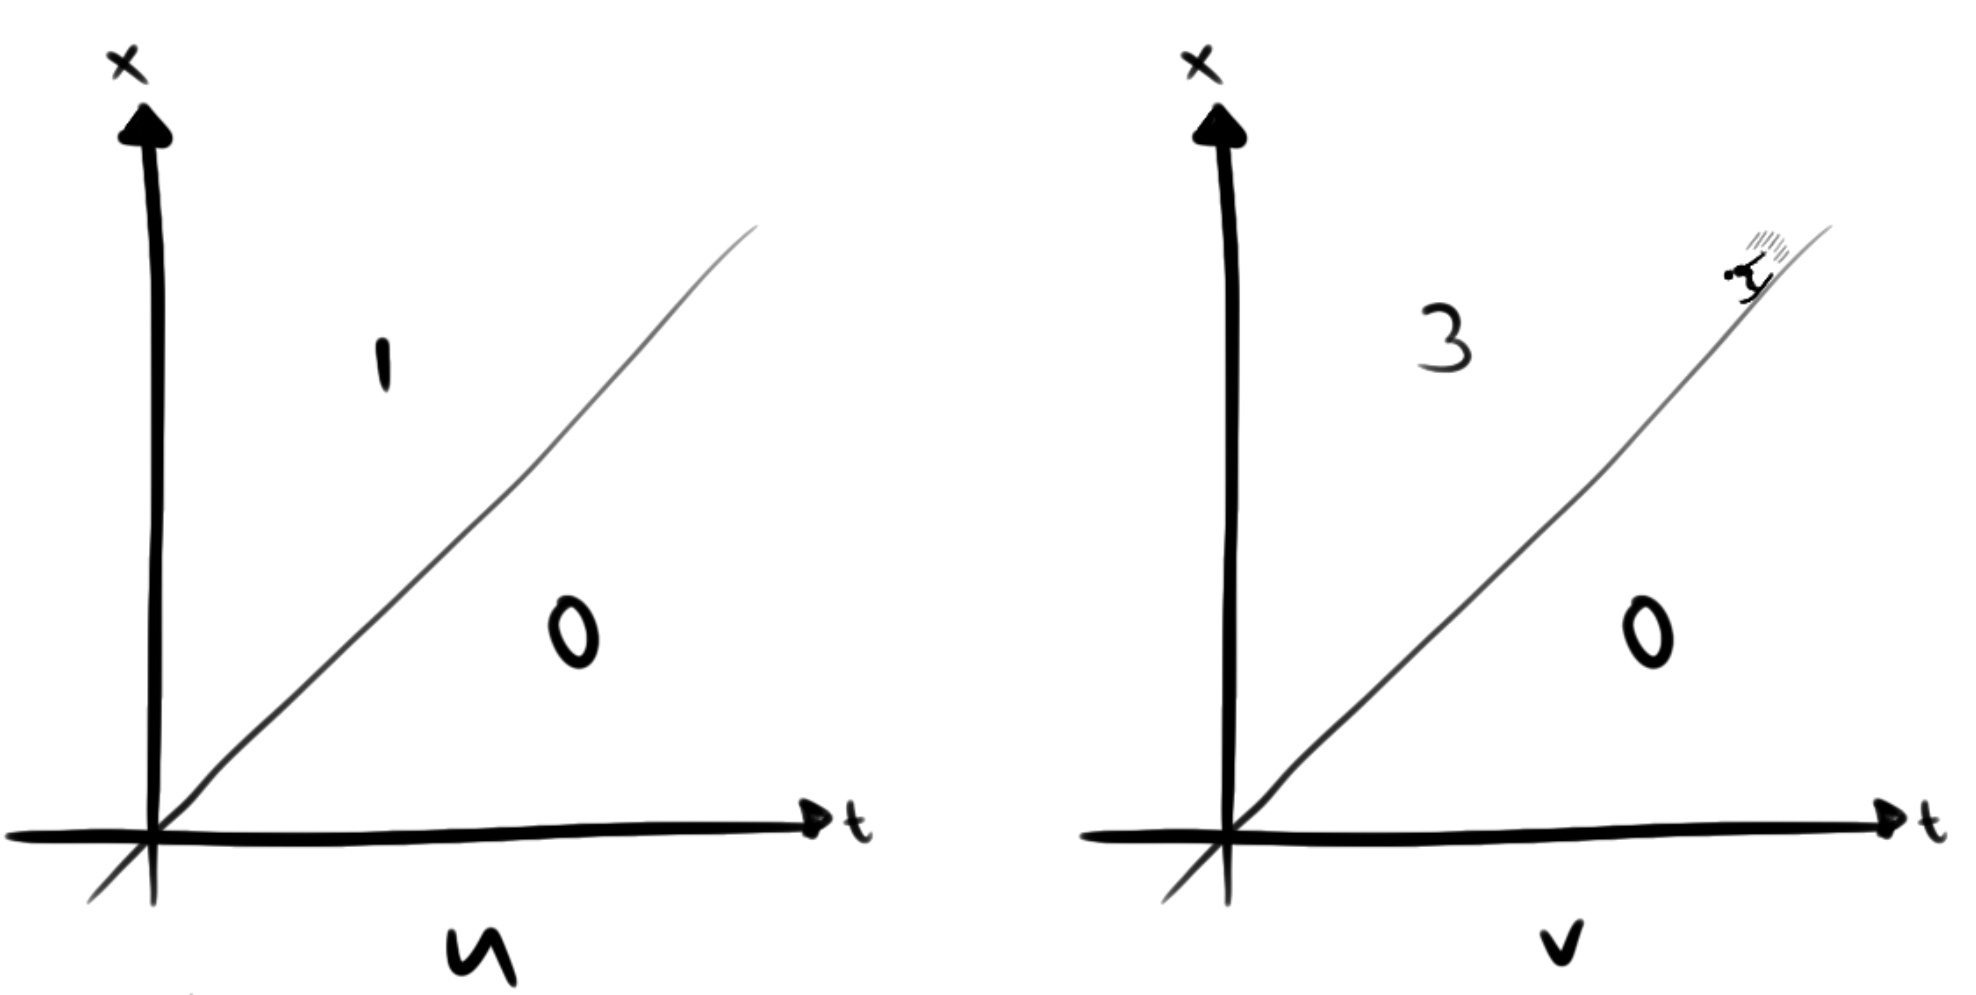
\includegraphics[height=3cm]{../images/uv}
    \end{center}
\end{enumerate}
\end{document}